%; whizzy paragraph -pdf xpdf -latex ./whizzypdfptex.sh
%; whizzy-paragraph "^\\\\begin{frame}"
% latex beamer presentation.
% platex, latex-beamer でコンパイルすることを想定。 

%     Tokyo Debian Meeting resources
%     Copyright (C) 2011 Junichi Uekawa
%     Copyright (C) 2011 Nobuhiro Iwamatsu

%     This program is free software; you can redistribute it and/or modify
%     it under the terms of the GNU General Public License as published by
%     the Free Software Foundation; either version 2 of the License, or
%     (at your option) any later version.

%     This program is distributed in the hope that it will be useful,
%     but WITHOUT ANY WARRANTY; without even the implied warreanty of
%     MERCHANTABILITY or FITNESS FOR A PARTICULAR PURPOSE.  See the
%     GNU General Public License for more details.

%     You should have received a copy of the GNU General Public License
%     along with this program; if not, write to the Free Software
%     Foundation, Inc., 51 Franklin St, Fifth Floor, Boston, MA  02110-1301 USA

\documentclass[cjk,dvipdfmx,12pt]{beamer}
\usetheme{Tokyo}
\usepackage{monthlypresentation}

%  preview (shell-command (concat "evince " (replace-regexp-in-string  "tex$" "pdf"(buffer-file-name)) "&")) 
%  presentation (shell-command (concat "xpdf -fullscreen " (replace-regexp-in-string "tex$" "pdf"(buffer-file-name)) "&"))
%  presentation (shell-command (concat "evince " (replace-regexp-in-string "tex$" "pdf"(buffer-file-name)) "&"))

%http://www.naney.org/diki/dk/hyperref.html
%日本語EUC系環境の時
\AtBeginDvi{\special{pdf:tounicode EUC-UCS2}}
%シフトJIS系環境の時
%\AtBeginDvi{\special{pdf:tounicode 90ms-RKSJ-UCS2}}

\title{GPG キーサインパーティ}
\subtitle{KOF 2011}
\author{Nobuhiro Iwamatsu iwamatsu@debian.org\\IRC nick: iwamatsu}
\date{2011年11月12日}
\logo{
\includegraphics[width=8cm]{image201111/logo-gnupg.png}}

\begin{document}

\frame{\titlepage{}}

\begin{frame}
  \begin{center}\large\bfseries
   俺達はなぜ、なぜキーサインをするのかっ!?\\\pause
  \Huge  \color{red}{はやくリア充になりたいから...}
  \end{center}
\end{frame}

\begin{frame}{自己紹介}
\begin{itemize}[<+->]

\item リア充 \\
GPG Web of Trust 部門 約120000人中 471位
\item 岩松 信洋 (@iwamatsu)
\item ksp-ja(key sign party-ja)メンバ
\item Debian 公式開発者 \\
bluetooth, mozc, OpenCV, Renesas SH4ポーター etc....
\item 普段は Linux kernel、glibc , ブートローダ(U-boot)を開発とか。
\item ステージ/ジュンク堂16:20 「Gitによるバージョン管理」サイン会 (岩松信洋)
\end{itemize}
\end{frame}

\begin{frame}
  \begin{itemize}[<+->]
    \item PGP/GPG は公開鍵暗号方式 $\rightarrow$ 公開鍵を誰かに保証してもらう必要がある
    \item しかし PGP/GPG には認証局が無い
    \begin{itemize}
      \item 自分が相手を信頼して、相手が自分を信頼する\\
            お前が信じるお前を信じろ
      \item これをPGP/GPGユーザで相互に行う $\rightarrow$ ネットワークが構築される $\rightarrow$ Web of Trust
      \item そして{\color{red}リア充}になる
    \end{itemize}
    \item 実際に会って、相手の公開鍵と公的ID(パスポート、運転免許証)を確認、そして署名=キーサイン
    \item 誰とも鍵交換してない GPG 署名なんて何の意味を持たない\\
          だって誰にも信頼されてないじゃない.....。
  \end{itemize}
\end{frame}


\begin{frame}{日本 GPG Web of Trust リア充ランキング}
\begin{itemize}[<+->]
\item GPG Web of Trust 部門 約120000人中 471位 とか言いましたが...
\item 日本でも上には上がいる....\\
144位 Kenshi Muto \\
222位 Junichi Uekawa \\
419位 GOTO Masanori \\
\end{itemize}
\end{frame}

\begin{frame}{日本 GPG Web of Trust リア充ランキング}
\begin{itemize}
\item GPG Web of Trust 部門 約120000人中 471位 とか言いましたが...
\item 日本でも上には上がいる....\\
144位 Kenshi Muto {\color{red}(Debian 公式開発者)}\\
222位 Junichi Uekawa {\color{red}(Debian 公式開発者)}\\
419位 GOTO Masanori {\color{red}(Debian 公式開発者)}\\
\end{itemize}
\end{frame}


\begin{frame}{世界 GPG Web of Trust リア充ランキング}
\begin{itemize}[<+->]
\item 世界だと...\\
1位 Peter Palfrader \\
2位 Noel Kothe \\
3位 Martin Michlmayr \\
4位 Benjamin Hill (Mako) \\
5位 Peter Palfrader \\
6位 Rene Engelhard \\
\end{itemize}
\end{frame}

\begin{frame}{世界 GPG Web of Trust リア充ランキング}
\begin{itemize}
\item 世界だと...\\
1位 Peter Palfrader  {\color{red}(Debian 公式開発者)}\\
2位 Noiel Kothe {\color{red}(Debian 公式開発者)}\\
3位 Martin Michlmayr {\color{red}(Debian 公式開発者)}\\
4位 Benjamin Hill (Mako) {\color{red}(Debian 公式開発者)}\\
5位 Peter Palfrader {\color{red}(Debian 公式開発者)}\\
6位 Rene Engelhard {\color{red}(Debian 公式開発者)}\\
\end{itemize}
\end{frame}

\begin{frame}{世界 GPG Web of Trust リア充ランキング}

\begin{center}\large\bfseries
\color{red}{ようするに、\sout{Debian} FLOSS 開発者はリア充ということ}\\
(但し保証はできません)
\end{center}
\end{frame}

\begin{frame}{使い所: 開発者}
\begin{itemize}
  \item 存在証明
  \begin{itemize}
    \item 公開サーバのアカウント認証など
  \end{itemize}
  \item ソフトウェアのリリース署名
  \begin{itemize}
    \item Debian、Ubuntu では必須
    \item パッケージへの署名、投票の署名...
  \end{itemize}
  \item おい、Linux カーネルでもGPGサインが必須になるらしいぞ
\end{itemize}
\end{frame}

\begin{frame}{使い所: ユーザ}
\begin{itemize}
  \item メールの署名/暗号化
  \item データファイルの署名
  \item ソフトウェアの改竄チェック
  \begin{itemize}
    \item リポジトリの署名チェック(apt, yum etc..)
  \end{itemize}
\end{itemize}
\end{frame}


\begin{frame}
  \begin{center}

これらを行うには Web of Trust に参加している必要がある \\ \pause
\Huge\bfseries 
というわけで、キーサインしましょう。
  \end{center}
\end{frame}


\begin{frame}{キーサインの流れ}
\begin{enumerate}
  \item キーサーバに自分の公開鍵をアップロード
  \item 相手の確認(名前、公開鍵の指紋, ID、メールアドレス)
  \item 相手の公開鍵に署名(メールアドレス毎に!)
  \item 署名した相手に公開鍵を送信(メールアドレス毎に!)
  \item 相手に署名された自分の鍵を取り込む
  \item キーサーバに自分の公開鍵をアップロード
\end{enumerate}
\end{frame}

\begin{frame}{SHA256 ハッシュ}
\begin{center}
本日のハッシュ\\
\Huge
a1b8 b5ae 30d0 ce07\\
b355 b6d8 e05d af4a\\
e813 1d9f bbc7 79d4\\
c9d2 03f9 6495 fac3\\

\end{center}
\end{frame}


\begin{frame}{キーサインパーティ前のWoT}
\begin{center}
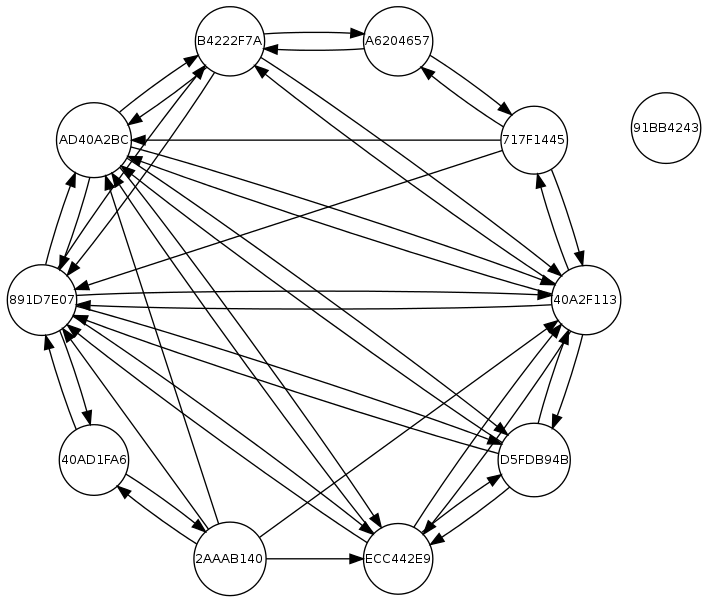
\includegraphics[width=0.8\hsize]{image201111/kof2011-ksp.png}
\end{center}
\end{frame}


\begin{frame}{キーサインパーティ後のWoT}
\begin{center}
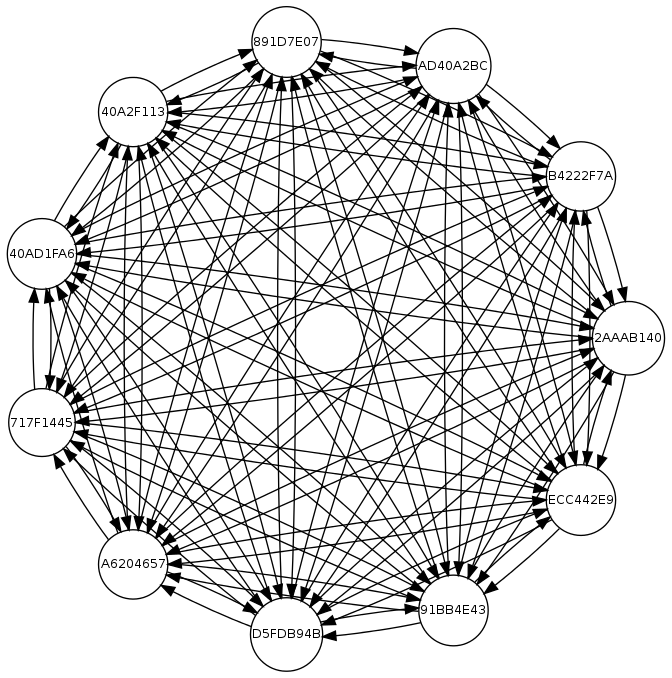
\includegraphics[width=0.7\hsize]{image201111/kof2011-ksp0.png}
\end{center}
\end{frame}

\begin{frame}{GPG サインパーティ後}

\begin{itemize}
\item 相手にサインして送るまでがGPGサイン。
\item caff を使うと楽ちんです。
\end{itemize}

\end{frame}

\begin{frame}{おしらせ}

\begin{itemize}
\item 6F/M6 13:00 なれる! Debian 開発者 ― 45 分でわかる?メンテナ入門(やまねひでき)
\item ステージ/ジュンク堂16:20 「Gitによるバージョン管理」サイン会 (岩松信洋)
\end{itemize}

\end{frame}


\end{document}

;;; Local Variables: ***
;;; outline-regexp: "\\([ 	]*\\\\\\(documentstyle\\|documentclass\\|emtext\\|section\\|begin{frame}\\)\\*?[ 	]*[[{]\\|[]+\\)" ***
;;; End: ***
